%%% Template originaly created by Karol Kozioł (mail@karol-koziol.net) and modified for ShareLaTeX use

\documentclass[a4paper,11pt]{article}

\usepackage[T1]{fontenc}
\usepackage[utf8]{inputenc}
\usepackage{graphicx}
\graphicspath{ {./images/} }

\usepackage{xcolor}

\renewcommand\familydefault{\sfdefault}
\usepackage{tgheros}

\usepackage{amsmath,amssymb,amsthm,textcomp,latexsym}
\usepackage{enumerate}
\usepackage{multicol}
\usepackage{tikz}

\usepackage{caption}
\usepackage{subcaption}
\usepackage{epstopdf}
\usepackage{cancel}
\usepackage{mathtools}


\usepackage{geometry}
\geometry{total={210mm,297mm},
left=25mm,right=25mm,%
bindingoffset=0mm, top=20mm,bottom=20mm}


\linespread{1.3}

\newcommand{\linia}{\rule{\linewidth}{0.5pt}}

% custom theorems if needed
\newtheoremstyle{mytheor}
    {1ex}{1ex}{\normalfont}{0pt}{\scshape}{.}{1ex}
    {{\thmname{#1 }}{\thmnumber{#2}}{\thmnote{ (#3)}}}

\theoremstyle{mytheor}
\newtheorem{defi}{Definition}

% my own titles
\makeatletter
\renewcommand{\maketitle}{
\begin{center}
\vspace{2ex}
{\huge \textsc{\@title}}
\vspace{1ex}
\\
\linia\\
\@author \hfill \@date
\vspace{4ex}
\end{center}
}
\makeatother
%%%

% custom footers and headers
\usepackage{fancyhdr}
\pagestyle{fancy}
\lhead{Projeto 1}
\chead{}
\rhead{2019.2}
\lfoot{}
\cfoot{}
\rfoot{Page \thepage}
\renewcommand{\headrulewidth}{0pt}
\renewcommand{\footrulewidth}{0pt}
%

% code listing settings
\usepackage{listings}
\lstset{
    language=Matlab,
    basicstyle=\ttfamily\small,
    aboveskip={1.0\baselineskip},
    belowskip={1.0\baselineskip},
    columns=fixed,
    extendedchars=true,
    breaklines=true,
    tabsize=4,
    prebreak=\raisebox{0ex}[0ex][0ex]{\ensuremath{\hookleftarrow}},
    frame=lines,
    showtabs=false,
    showspaces=false,
    showstringspaces=false,
    keywordstyle=\color[rgb]{0.627,0.126,0.941},
    commentstyle=\color[rgb]{0.133,0.545,0.133},
    stringstyle=\color[rgb]{01,0,0},
    numbers=left,
    numberstyle=\small,
    stepnumber=1,
    numbersep=10pt,
    captionpos=t,
    escapeinside={\%*}{*)}
}

%%%----------%%%----------%%%----------%%%----------%%%


\DeclarePairedDelimiter\abs{\lvert}{\rvert}%
\DeclarePairedDelimiter\norm{\lVert}{\rVert}%

% Swap the definition of \abs* and \norm*, so that \abs
% and \norm resizes the size of the brackets, and the 
% starred version does not.
\makeatletter
\let\oldabs\abs
\def\abs{\@ifstar{\oldabs}{\oldabs*}}
%
\let\oldnorm\norm
\def\norm{\@ifstar{\oldnorm}{\oldnorm*}}
\makeatother

\begin{document}

\title{Robótica e Automação}

\author{Raphael Barros Parreira}

\date{}

\maketitle

\section{Controle Cinemático de Manipuladores} % 1

\subsection{Controle}

De acordo com a tabela de Denavit Hartenberg Standard, o manipulador Antropomórfico 6R possui um punho equivalente a um punho esférico, cujo tamanho dos elos é 0. Isto significa que as 3 últimas juntas não influenciam na posição do efetuador. O objetivo deste exercício é controlar a posição do efetuador dados 3 trajetórias, e nada é pedido em relação à orientação do manipulador. Portanto iremos trabalhar com um sistema reduzido em que apenas as 3 primeiras juntas serão controladas (as outras três juntas permanecerão na posição ready).

No controle cinemático assume-se que a velocidade do manipulador é a variável manipulada.

\begin{gather*}
J = \begin{bmatrix} J_p \\ J_o \end{bmatrix} \qquad
\begin{bmatrix} \vec{v} \\ \vec{\omega} \end{bmatrix} = J\dot{\theta} = Ju
= \begin{bmatrix}J_pu \\ J_ou\end{bmatrix} \\
u = \begin{bmatrix}u_{13} \\ u_{46}\end{bmatrix} \qquad
J_p = \begin{bmatrix}J_{p13} & J_{p46}\end{bmatrix} \\
\vec{v} = J_{p13}u_{13} + J_{46}u_{46}
\end{gather*}

\begin{gather*}
\norm{J^\dagger}_{max} = 4.277 \qquad
\norm{\dot{x}_d}_{max} = 0.2356 \qquad
\norm{e}_{max} = 0.1417 \\
K_{base} \approx \dfrac{\dfrac{3}{\norm{J^\dagger}_{max}} - \norm{\dot{x}_d}_{max}}{\norm{e}_{max}} \approx 3.3
\end{gather*}

\begin{table}[!ht]
\centering
\caption{Ganhos para os controles com e sem Feed-forward em todas as 3 trajetórias.}
\label{tab:ex5_ikine_configuracao}

\begin{tabular}{|c|c|c|}
\hline
Controles  & FB & FF \\ \hline
Trajetória 1     & $8.91$ & $7.24$ \\ \hline
Trajetória 2     & $8.91$ & $8.57$ \\ \hline
Trajetória 3     & $8.91$ & $8.57$ \\ \hline
\end{tabular}
\end{table}


\begin{figure}[!ht]
\centering
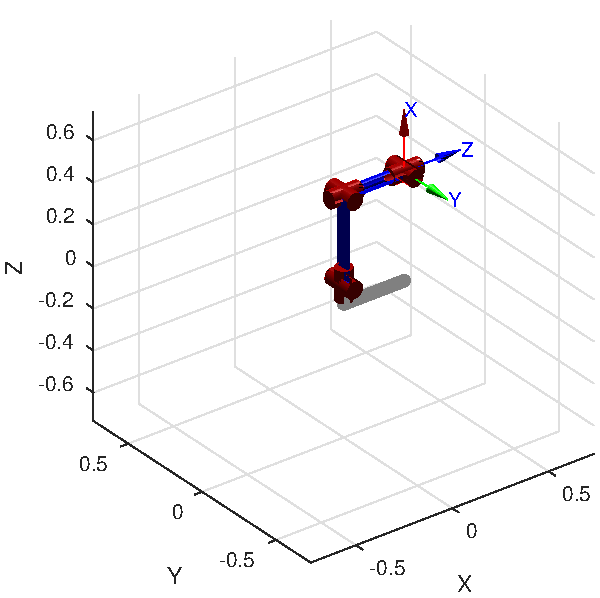
\includegraphics[width=1\textwidth]{figs/ex1_ready.pdf}
\caption{Ex 1: Manipulador Antropomórfico na posição ready}
\label{fig:ex1_ready}
\end{figure}

\begin{figure}[!ht]
\centering
  \begin{minipage}{\linewidth}
  \centering
    \begin{subfigure}[b]{1\textwidth}
    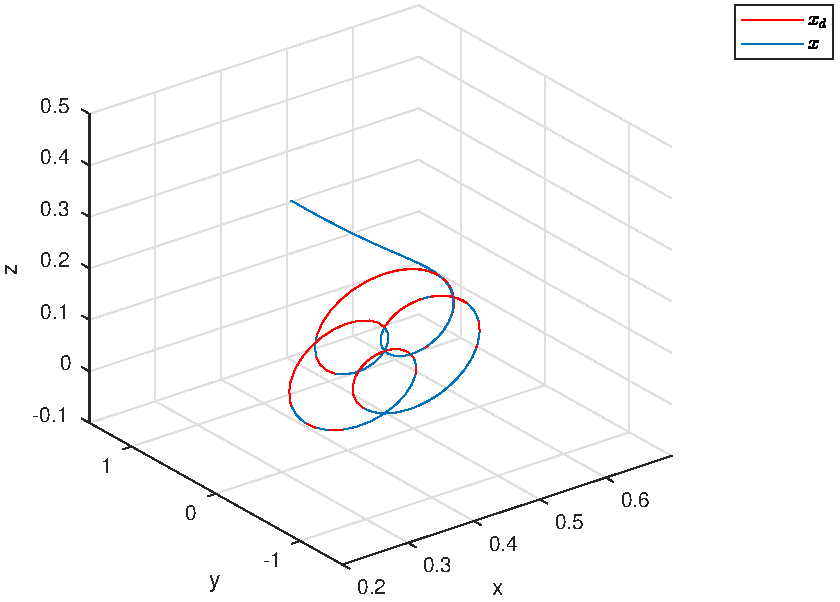
\includegraphics[width=1\textwidth]{figs/ex1_a_1_x.pdf}
    \caption{$x_d$ e $x$}
    \label{fig:ex1_a_1_x}
    \end{subfigure}
  \end{minipage}
  \begin{minipage}{\linewidth}
  \centering
    \begin{subfigure}[b]{0.45\textwidth}
    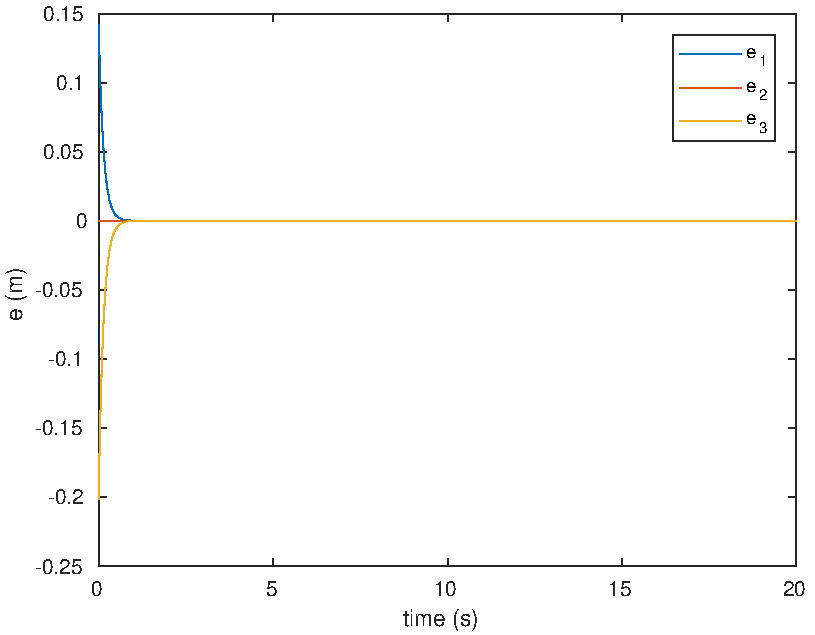
\includegraphics[width=1\textwidth]{figs/ex1_a_1_e.pdf}
    \caption{$e = x_d - x$}
    \label{fig:ex1_a_1_e}
    \end{subfigure}
    \begin{subfigure}[b]{0.45\textwidth}
    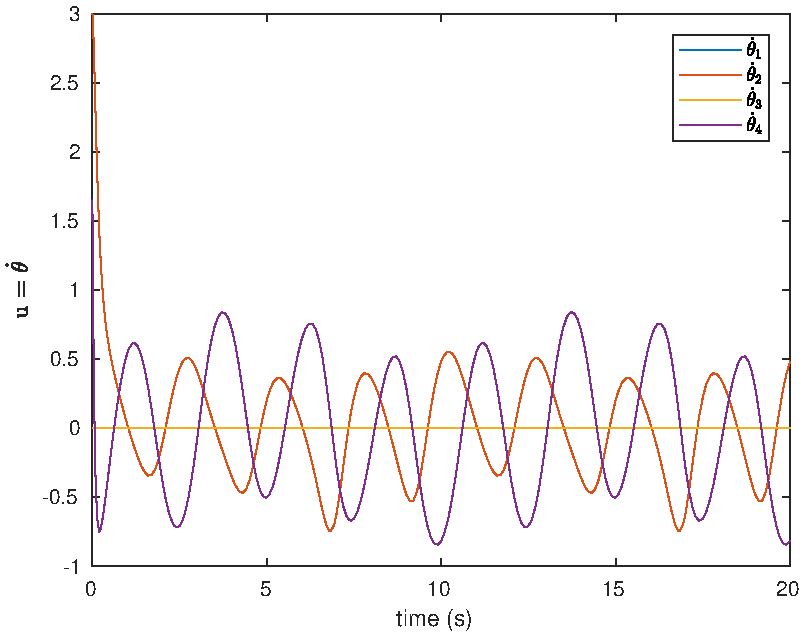
\includegraphics[width=1\textwidth]{figs/ex1_a_1_dq.pdf}
    \caption{$u = \dot{\theta}$}
    \label{fig:ex1_a_1_dq}
    \end{subfigure}
  \end{minipage}
\caption{Ex 1: Trajetória $a$, controle com FF.}
\label{fig:ex1_a_1}
\end{figure}


\begin{figure}[!ht]
\centering
  \begin{minipage}{\linewidth}
  \centering
    \begin{subfigure}[b]{1\textwidth}
    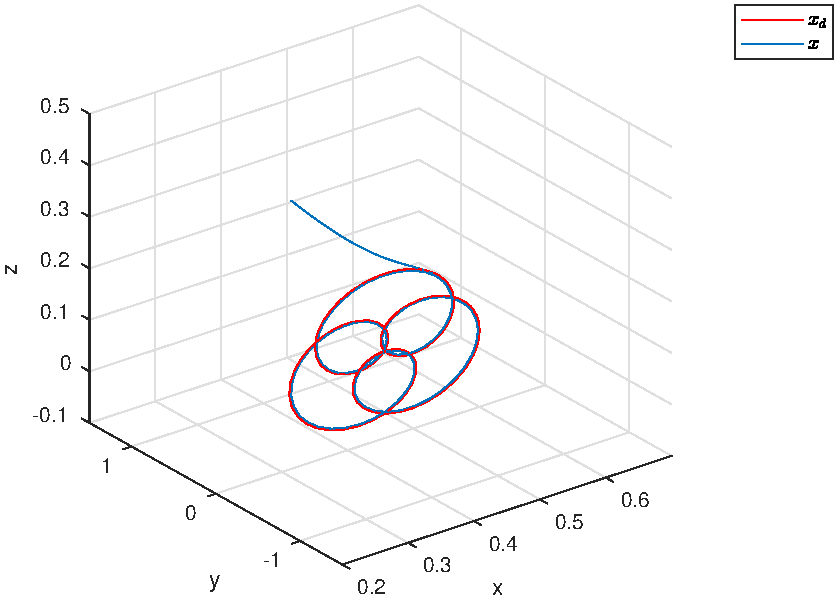
\includegraphics[width=1\textwidth]{figs/ex1_a_2_x.pdf}
    \caption{$x_d$ e $x$}
    \label{fig:ex1_a_2_x}
    \end{subfigure}
  \end{minipage}
  \begin{minipage}{\linewidth}
  \centering
    \begin{subfigure}[b]{0.45\textwidth}
    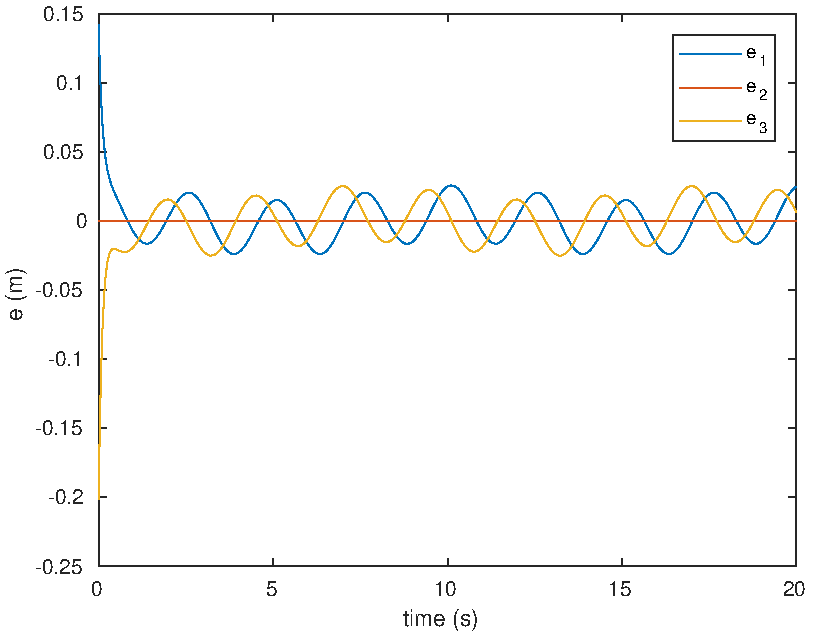
\includegraphics[width=1\textwidth]{figs/ex1_a_2_e.pdf}
    \caption{$e = x_d - x$}
    \label{fig:ex1_a_2_e}
    \end{subfigure}
    \begin{subfigure}[b]{0.45\textwidth}
    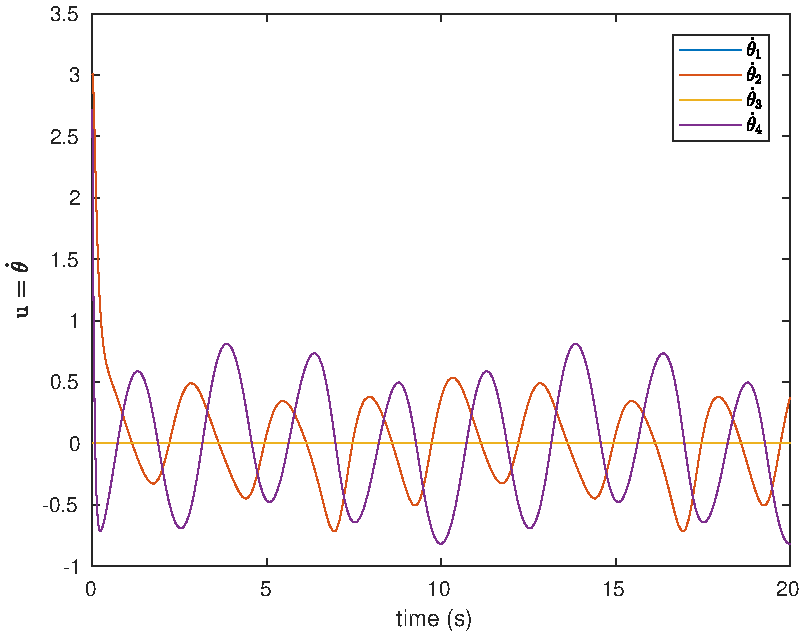
\includegraphics[width=1\textwidth]{figs/ex1_a_2_dq.pdf}
    \caption{$u = \dot{\theta}$}
    \label{fig:ex1_a_2_dq}
    \end{subfigure}
  \end{minipage}
\caption{Ex 1: Trajetória $a$, controle sem FF.}
\label{fig:ex1_a_2}
\end{figure}


\begin{figure}[!ht]
\centering
  \begin{minipage}{\linewidth}
  \centering
    \begin{subfigure}[b]{1\textwidth}
    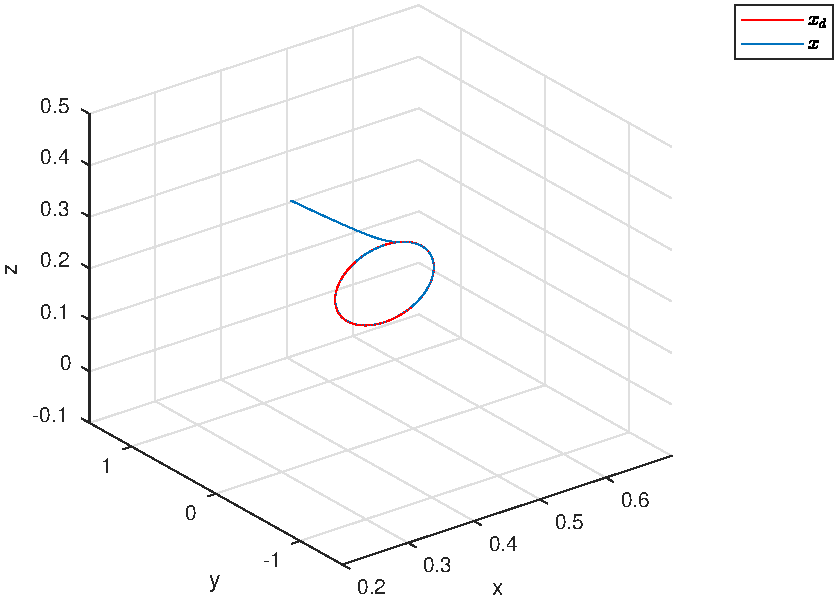
\includegraphics[width=1\textwidth]{figs/ex1_b_2_x.pdf}
    \caption{$x_d$ e $x$}
    \label{fig:ex1_b_2_x}
    \end{subfigure}
  \end{minipage}
  \begin{minipage}{\linewidth}
  \centering
    \begin{subfigure}[b]{0.45\textwidth}
    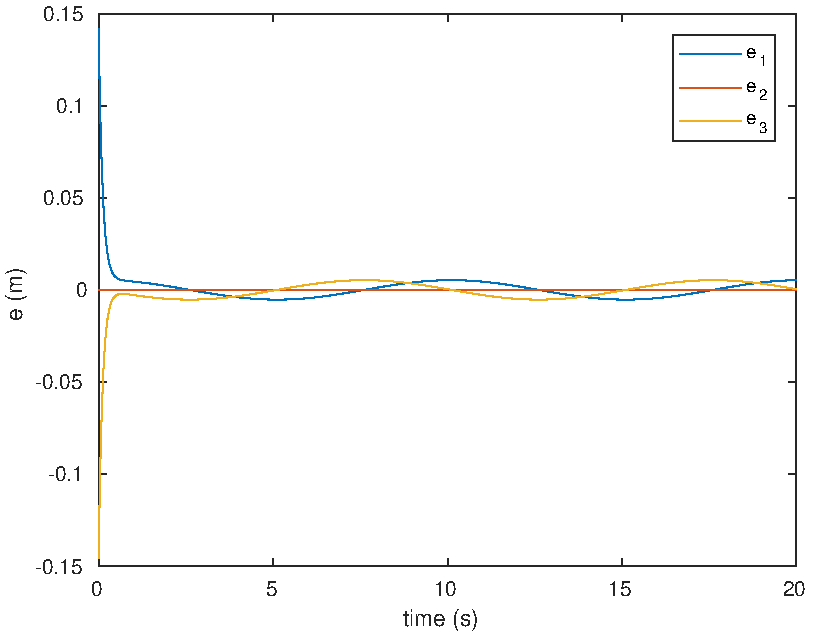
\includegraphics[width=1\textwidth]{figs/ex1_b_2_e.pdf}
    \caption{$e = x_d - x$}
    \label{fig:ex1_b_2_e}
    \end{subfigure}
    \begin{subfigure}[b]{0.45\textwidth}
    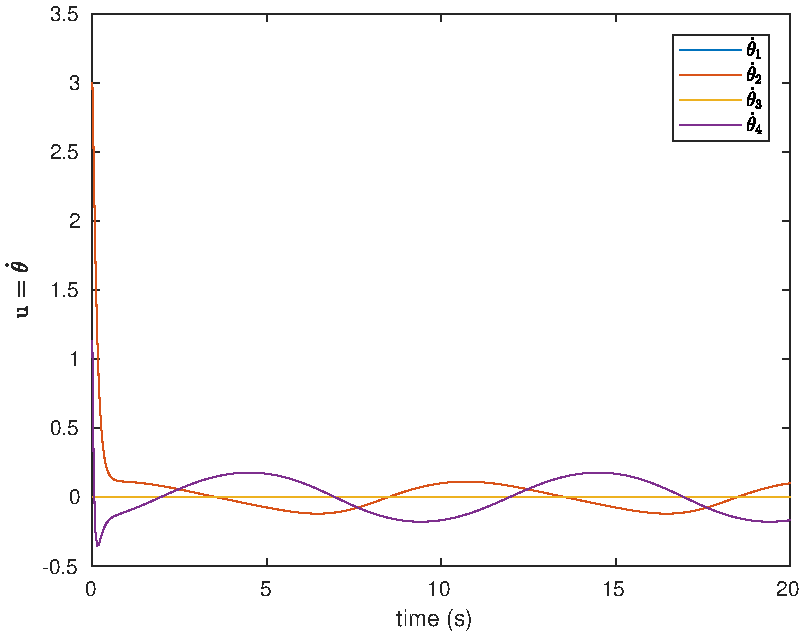
\includegraphics[width=1\textwidth]{figs/ex1_b_2_dq.pdf}
    \caption{$u = \dot{\theta}$}
    \label{fig:ex1_b_2_dq}
    \end{subfigure}
  \end{minipage}
\caption{Ex 1: Trajetória $b$, controle sem FF.}
\label{fig:ex1_b_2}
\end{figure}


\begin{figure}[!ht]
\centering
  \begin{minipage}{\linewidth}
  \centering
    \begin{subfigure}[b]{1\textwidth}
    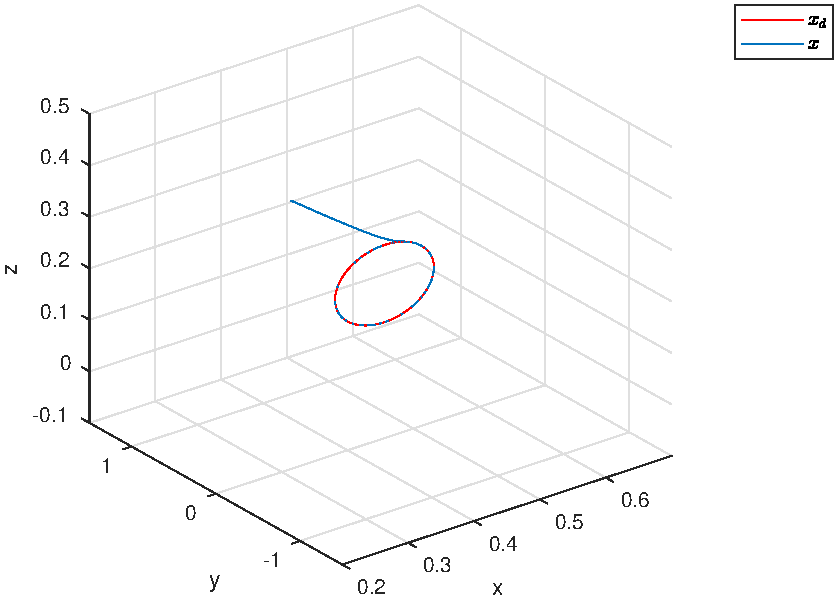
\includegraphics[width=1\textwidth]{figs/ex1_b_1_x.pdf}
    \caption{$x_d$ e $x$}
    \label{fig:ex1_b_1_x}
    \end{subfigure}
  \end{minipage}
  \begin{minipage}{\linewidth}
  \centering
    \begin{subfigure}[b]{0.45\textwidth}
    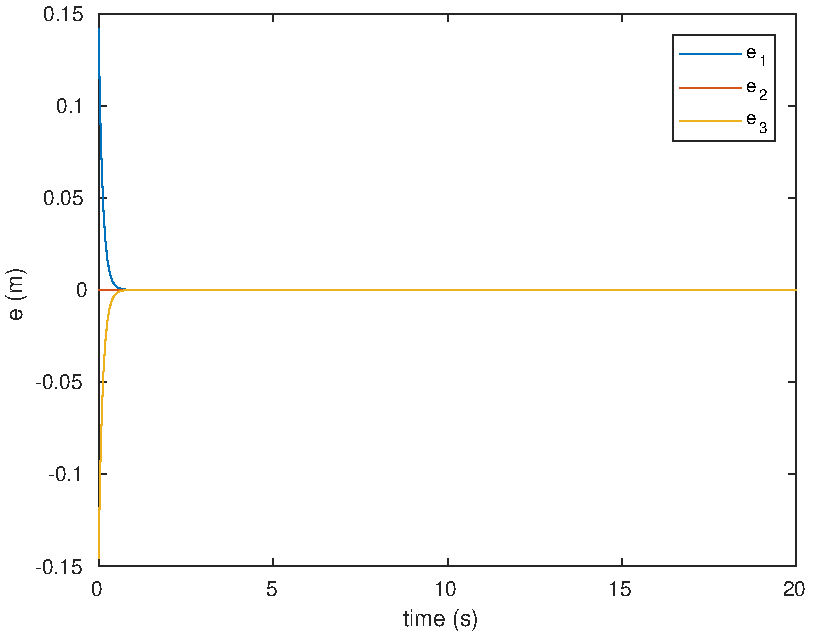
\includegraphics[width=1\textwidth]{figs/ex1_b_1_e.pdf}
    \caption{$e = x_d - x$}
    \label{fig:ex1_b_1_e}
    \end{subfigure}
    \begin{subfigure}[b]{0.45\textwidth}
    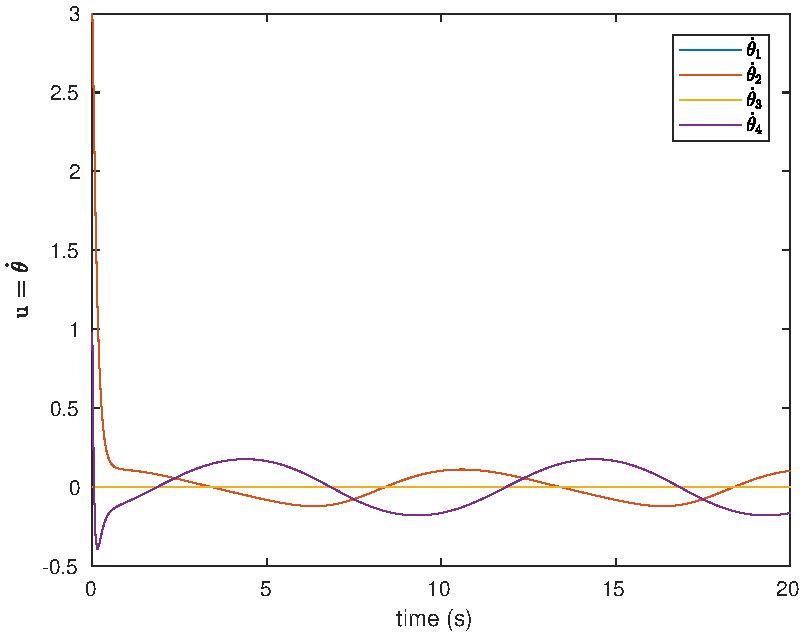
\includegraphics[width=1\textwidth]{figs/ex1_b_1_dq.pdf}
    \caption{$u = \dot{\theta}$}
    \label{fig:ex1_b_1_dq}
    \end{subfigure}
  \end{minipage}
\caption{Ex 1: Trajetória $b$, controle com FF.}
\label{fig:ex1_b_1}
\end{figure}


\begin{figure}[!ht]
\centering
  \begin{minipage}{\linewidth}
  \centering
    \begin{subfigure}[b]{1\textwidth}
    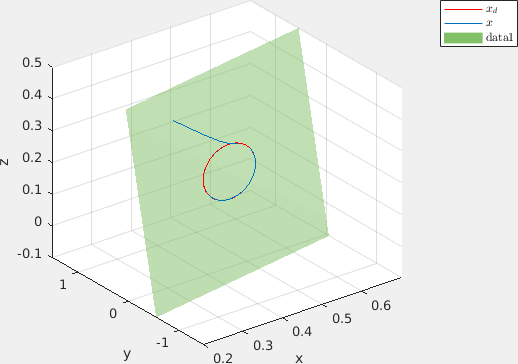
\includegraphics[width=1\textwidth]{figs/ex1_c_2_x.png}
    \caption{$x_d$ e $x$}
    \label{fig:ex1_c_2_x}
    \end{subfigure}
  \end{minipage}
  \begin{minipage}{\linewidth}
  \centering
    \begin{subfigure}[b]{0.45\textwidth}
    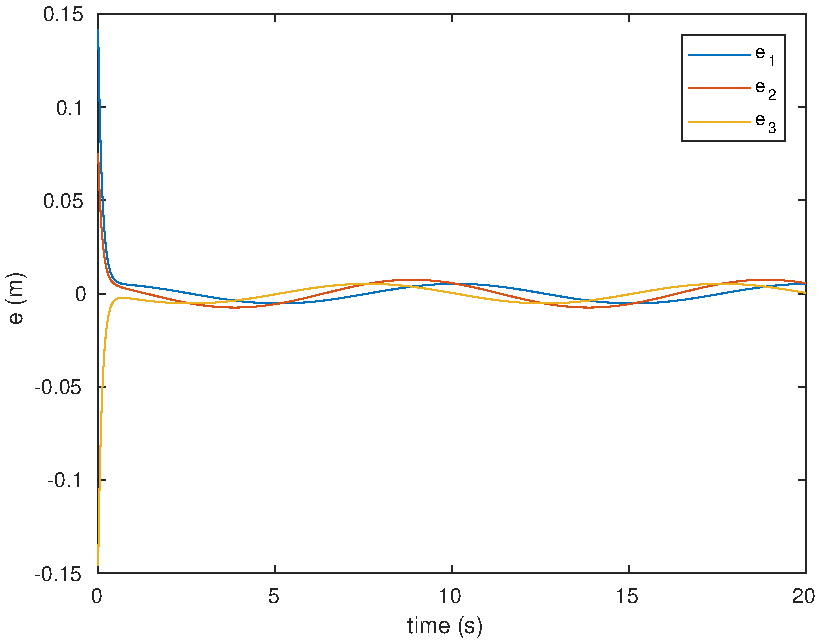
\includegraphics[width=1\textwidth]{figs/ex1_c_2_e.pdf}
    \caption{$e = x_d - x$}
    \label{fig:ex1_c_2_e}
    \end{subfigure}
    \begin{subfigure}[b]{0.45\textwidth}
    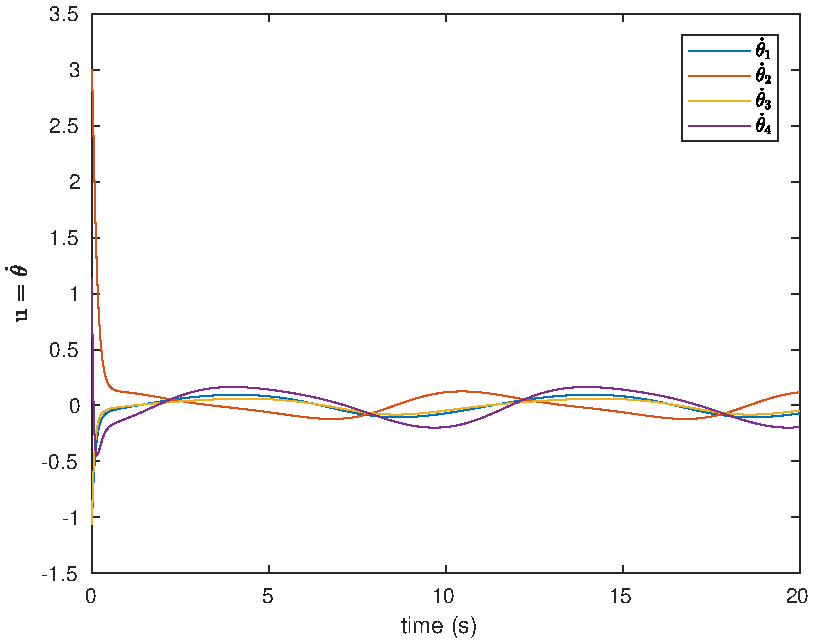
\includegraphics[width=1\textwidth]{figs/ex1_c_2_dq.pdf}
    \caption{$u = \dot{\theta}$}
    \label{fig:ex1_c_2_dq}
    \end{subfigure}
  \end{minipage}
\caption{Ex 1: Trajetória $c$, controle sem FF.}
\label{fig:ex1_c_2}
\end{figure}


\begin{figure}[!ht]
\centering
  \begin{minipage}{\linewidth}
  \centering
    \begin{subfigure}[b]{1\textwidth}
    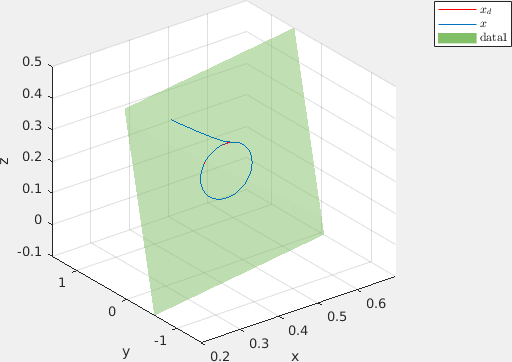
\includegraphics[width=1\textwidth]{figs/ex1_c_1_x.png}
    \caption{$x_d$ e $x$}
    \label{fig:ex1_c_1_x}
    \end{subfigure}
  \end{minipage}
  \begin{minipage}{\linewidth}
  \centering
    \begin{subfigure}[b]{0.45\textwidth}
    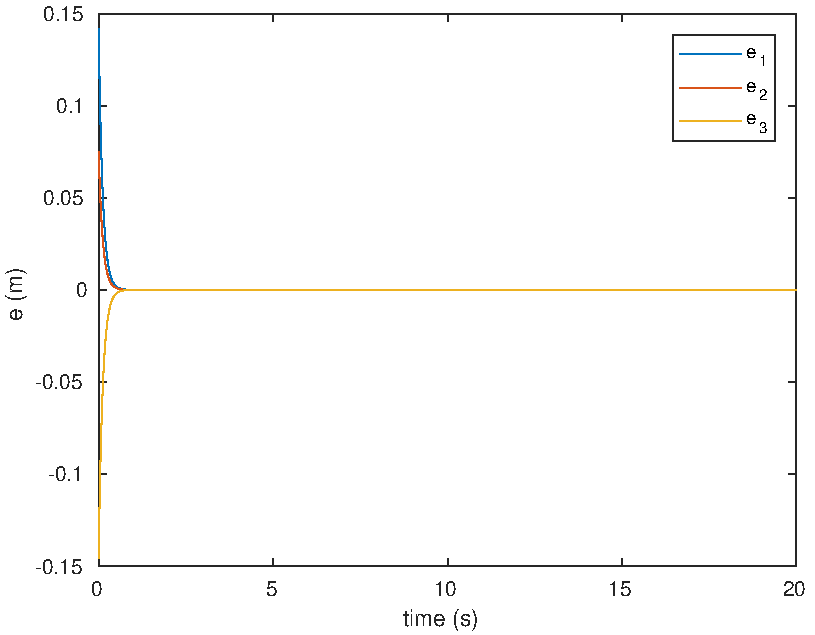
\includegraphics[width=1\textwidth]{figs/ex1_c_1_e.pdf}
    \caption{$e = x_d - x$}
    \label{fig:ex1_c_1_e}
    \end{subfigure}
    \begin{subfigure}[b]{0.45\textwidth}
    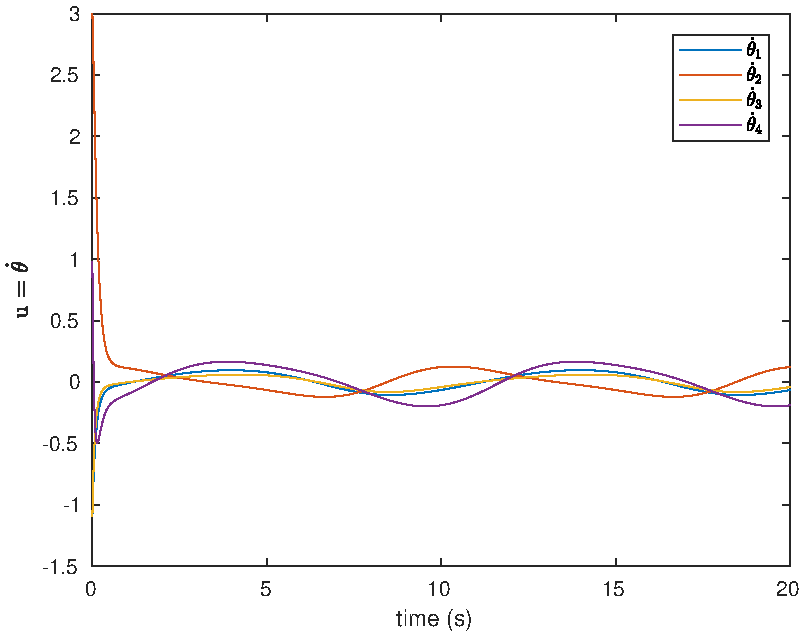
\includegraphics[width=1\textwidth]{figs/ex1_c_1_dq.pdf}
    \caption{$u = \dot{\theta}$}
    \label{fig:ex1_c_1_dq}
    \end{subfigure}
  \end{minipage}
\caption{Ex 1: Trajetória $c$, controle com FF.}
\label{fig:ex1_c_1}
\end{figure}

Como as dimensões dos últimos 3 elos são 0, o $J_{p46}$ será sempre $\begin{bmatrix}0 & 0 & 0\end{bmatrix}^T$, portanto trabalharemos com um sistema reduzido com $J_{p46}$. Também é preciso escolher uma base para expressar os vetores. Como a trajetória desejada é descrita no sistema inercial, o sistema também será descrito no sistema inercial.

\begin{gather*}
\vec{v} = \dot{\vec{x}} = J_{p13}u_{13}
\end{gather*}

Escolhendo trabalhar no sistema inercial teremos:

\begin{gather*}
(\vec{v})_0 = v = \dot{x} = (J_{p13})_0u_{13}
\end{gather*}

Pelo enunciado é preciso realizar o controle com duas formulações para $u_{13}$, uma que use o inverso de $J_{p13}$ e outro com a transposta de $J_{p13}$.

\begin{gather*}
u_{1} = (J_{p13})_0^{-1}\bar{u} = (J_{p13})_0^{-1}(\dot{x}_d + K(x_d - x)) \\
u_{2} = (J_{p13})_0^T\bar{u} = (J_{p13})_0^T(\alpha\dot{x}_d + K(x_d - x))
\end{gather*}

Justificativa para $u_{2}$ com $\alpha \neq 0$? Não consegui encontrar uma função de Lyapunov que garanta $\dot{V} \leq 0$. Podemos provar que $u_{2}$ torna o sistema assintoticamente estável para o caso em que a trajetória desejada é uma constante ($\alpha = 0$), mas como as trajetórias desejadas do enunciado são variantes no tempo  não podemos garantir $\dot{V} \leq 0$, ou seja, $u_{2}$ com $\alpha = 0$ não consegue zerar o erro para as trajetórias desejadas. No caso da trajetória constante temos:

\begin{gather*}
2V = e^Te \\
\dot{V} = e^T\dot{e} = e^T(\dot{x}_d - \dot{x}) = e^T(\dot{x}_d - (J_{p13})_0u) = \\ = e^T(\dot{x}_d - (J_{p13})_0(J_{p13})_0^T(\alpha \dot{x}_d + Ke)) \\
\dot{x}_d = 0 \implies \dot{V} = -e^T(J_{p13})_0(J_{p13})_0^TKe = -K(e^T(J_{p13})_0)(e^T(J_{p13})_0)^T \\
\dot{V} \leq 0
\end{gather*}


Para verificar os resultados obtidos pelas multiplicações da questão 6. Foi usada a função \textit{SerialLink.jacob0}. Os resultados estão na figura \ref{fig:ex6_verif}.

As duas figuras mostram que os resultados obtidos não estão corretos.


\end{document}
